\documentclass[conference]{IEEEtran}
\usepackage{cite}
\usepackage{amsmath,amssymb,amsfonts}
\usepackage{algorithmic}
\usepackage{graphicx}
\usepackage{textcomp}
\usepackage{xcolor}
\def\BibTeX{{\rm B\kern-.05em{\sc i\kern-.025em b}\kern-.08em
    T\kern-.1667em\lower.7ex\hbox{E}\kern-.125emX}}
\begin{document}

\title{Nanuda: A Group Expenses Manager}

\author{\IEEEauthorblockN{1\textsuperscript{st} Abia Herlianto}
\IEEEauthorblockA{\textit{School of Computer Science} \\
\textit{BINUS University}\\
\textit{Team MONEY}\\
Jakarta, Indonesia \\
abiaph@live.com}
\and
\IEEEauthorblockN{2\textsuperscript{nd} Hugo Ravé}
\IEEEauthorblockA{\textit{General Engineering} \\
\textit{ESILV PARIS-LA DEFENSE}\\
\textit{Team MONEY}\\
Paris, France \\
hugorave07@gmail.com}
\and
\IEEEauthorblockN{3\textsuperscript{rd} Nadya Hartanto}
\IEEEauthorblockA{\textit{School of Information Systems} \\
\textit{BINUS University}\\
\textit{Team MONEY}\\
Jakarta, Indonesia \\
ndhartanto1@gmail.com}
}

\maketitle

\begin{abstract}
Users create a "group" composed of either one person (themselves) or several people. Users then invite these people to the group. Users add expenses and split the costs with either all, some, or no members of the group. Users can categorise and add descriptions for each expense. Users can also customise how the costs are split. Users can see a summary of how much they owe to others and how much others owe to others. The summary of how much users owe changes as users spend and pay.
\end{abstract}

\begin{IEEEkeywords}
expenses, finance, management
\end{IEEEkeywords}

\begin{center}
\begin{tabular}{|p{6em}|p{5em}|p{10em}|}
\hline
\textbf{Role} & \textbf{Name} & \textbf{Task Description etc.} \\
\hline
\textbf{User/Customer} & Nadya Hartanto & Tests the application for bugs and issues. Provides feedback to the Development Manager.
Also provides feedback on UX and UI quality. \\
\hline
\textbf{Software Developer} & Abia Putrama Herlianto & Implements software based on design. Fixes bugs and issues. \\
\hline
\textbf{Development Manager} & Hugo Ravé & Designs software based on requirements and feedback from User/Customer. Organises, schedules, and manages development. \\
\hline
\end{tabular}
\end{center}

\section{Introduction}
When there are shared expenses in a group, it can be complicated to split the costs and gather the money that each person should pay. The usual solution is to have one or several individuals cover the cost of the entire group, and from there the remaining group members would pay their share to those who covered the cost.

The problem that arises from this is keeping track of these expenses. This is especially true for groups that meet regularly; for example, a group of friends going on a trip. Keeping track of who covered what for how much and who owes whom how much can quickly get out of hand. The solution that we propose is a simple application where these expenses can be organised, viewed, and accessed by all members of a certain group.

The name Nanuda comes from Korean 나누다, meaning 'to divide (up), to split (up)'. The name was chosen because our own experiences in splitting expenses in Korea was the reason we thought up of the idea.

There are several existing applications that perform a similar function, with different individual features. These include Tricount and Sesterce.
\begin{enumerate}
    \item \textbf{Tricount}
        \begin{figure}[htbp]
            \centerline{
\includegraphics[width=50mm,scale=0.5]{img/logo-tricount.png}}
            \caption{Tricount}
            \label{fig:my_label}
        \end{figure}
        \\
        (Data from Google Play Store) \\
        Rating: 4.8 stars \\
        Downloads: 1 million+ \\
        Key features: Users can share a simple link to share their expenses. Members of a group can add expenses and see the balance. Expenses can be shared unevenly. Tricount works both offline and online, with logging in being optional. It also has both a mobile app and a website.
    \item \textbf{Sesterce}
        \begin{figure}[htbp]
            \centerline{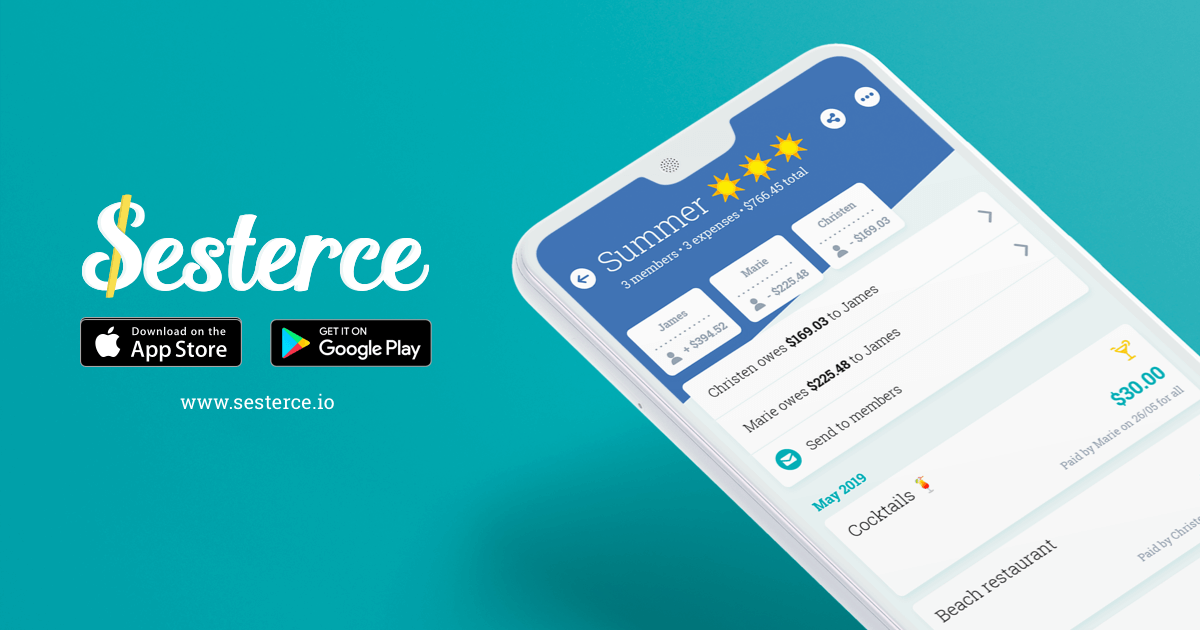
\includegraphics[width=50mm,scale=0.5]{img/logo-sesterce.png}}
            \caption{Sesterce}
            \label{fig:my_label}
        \end{figure}
        \\
        (Data from Google Play Store) \\
        Rating: 4.7 stars \\
        Downloads: 5,000+ \\
        Key features: Similar to Tricount, users can join a single group and add expenses, keeping track of all bills and costs. Sesterce is completely anonymous with no login or email required. In addition, Sesterce allows the addition of custom categories for expenses, the option to view statistics, and exporting all the data to a .csv file.
\end{enumerate}

\section{Requirements}

\begin{enumerate}
    \item \textbf {Loading Screen}: When the user opens the application, the loading screen will be displayed until the application has completed loading all the data from the server.
    \item \textbf {Groups}: If there are existing groups, their names and brief descriptions will be displayed. If it is the first time the application has been opened, a sample group will be present. The user can add another group by using the add group button. The user can enter an existing group by clicking on it. The user can also modify and delete existing groups by long-pressing the group which will display a "Group Details" pop-up.
    \begin{enumerate}
        \item \textbf{Enter Group}: The user can enter an existing group by clicking the group in the list.
        \item \textbf{Add Group}: Two options will be displayed. The user can join an group or make a new one.
            \begin{enumerate}
                \item\textbf {Make New Group}: A "New Group" form will be displayed. The user must input the name of the group, the currency used, and the names of the participants. The user can also optionally write a brief description of the group. The user can copy the link to the group for other participants to join the group.
                \item\textbf {Join Group}: A "Join Group" form will be displayed. The user must input a valid link of an existing group.
            \end {enumerate}
        \item \textbf{Edit Group}: An "Edit Group" form will be displayed. Similar to a "New Group" form, the user can change the name of the group, the currency used, and the number and names of the participants.
        \item \textbf{Delete Group}: The user can delete the group.
    \end{enumerate}
    \item \textbf {Expenses}: If there are existing expenses, the name of the expense, the amount, and the date will be displayed. All participants in the group can see the expenses list and add another expense by clicking the "Add Expense" button. The user can also see the details of an expense by clicking on it.
    \begin{enumerate}
        \item\textbf {Add Expense}: An "Add Expense" form will be displayed. The user must input the title, amount, date, category, payer participant, and paid for participants of the expense. Users can split the expense equally automatically by default or edit the amounts manually by percentage or by amount.
        \item\textbf {Expense Detail}: The details of the expense will be displayed: the title, amount, date, payer participant, and paid for participants. The exact amount each paid for participant owes for this expense is also displayed. Users can also edit this expense by clicking the "Edit" button and delete the expense by clicking the "Delete" button.
        \begin{enumerate}
            \item \textbf {Edit Expense}: An "Edit Expense" form will be displayed Similar to a "New Expense" form, the user can edit the title, amount, date, payer participant, and paid for participants.
            \item \textbf {Delete Expense}: The user can delete the expense.
        \end{enumerate}
    \end{enumerate}
    \item \textbf {Balances}: A summary of how much is owed will be displayed. The information on who owes whom how much is also displayed e.g. A owes B 3 dollars, A owes C 7 dollars, C owes B 2 dollars. The total amount of money owed or owed to for each participant is listed e.g. in total, A owes 10 dollars, B is owed 5 dollars, C is owed 5 dollars. C is owed 5 dollars because A owes C 7 dollars, but C owes B 2 dollars.
\end{enumerate}

\section{Development Environment}
\subsection{Choice of Software Development Platform}
\begin{enumerate}
    \item \textbf{Platform}
        \newline
        \begin{figure}[htbp]
            \centerline{
\includegraphics[width=50mm,scale=0.5]{img/logo-android.png}}
            \caption{Android}
            \label{fig:my_label}
        \end{figure}
        \newline
        For Nanuda, we have chosen the \textbf{Android} mobile operating system as the platform for several reasons:
        \begin{enumerate}
            \item Nanuda needs to be on a mobile platform for quick access and easy use
            \item Android is the best-selling mobile OS worldwide
            \item Resources for development on Android are widely available and at no cost
        \end{enumerate}
        
    \item \textbf{Programming Language}
        \newline
        \begin{figure}[htbp]
            \centerline{
\includegraphics[height=25mm,scale=0.5]{img/logo-java.png}}
            \caption{Java}
            \label{fig:my_label}
        \end{figure}
        \newline
        For the development of Nanuda, we use the \textbf{Java} programming language. Java is a class-based, object-oriented programming language and one of the world's most popular and widely used programming languages. We chose to use Java for two reasons:
        \begin{enumerate}
            \item Java is the language used to develop Android apps through the Android SDK
            \item We are familiar with Java and have used it in the past
        \end{enumerate}
    \item \textbf{Cost Estimation}
        \newline
        For the development of Nanuda, all of the resources used are either free of charge or have both free and paid options. For the resources with free and paid options, we have decided to use the free option. As such, the development of Nanuda requires no cost.
        \begin{center}
            \begin{tabular}{|p{6em}|p{10em}|p{4em}|}
                \hline
                \textbf{Resource} & \textbf{Role Description} & \textbf{Cost} \\
                \hline
                Android Studio & Android Development IDE & 0 \\
                \hline
                AWS Educate & Backend Server & 0 \\
                \hline
                Overleaf & Online, Collaborative LaTeX Writing Tool & 0 \\
                \hline
                GitHub & Remote Repository and Version Control System & 0 \\
                \hline
                GitHub Desktop & GUI for GitHub & 0 \\
                \hline
            \end{tabular}
        \end{center}
    \item \textbf{Development Environment}
    \begin{itemize}
        \item \textbf{Android Studio Version 4.1} \\
        Android Studio was chosen because it is the official IDE for the Android operating system.
        \item \textbf{AWS Educate} \\
        AWS Educate is Amazon's programme for students to use AWS services at no cost.
        \item \textbf{Overleaf} \\
        Overleaf was chosen because of its popularity and the effectiveness of its features, namely simple, in-browser editing, immediate compilation, easy sharing and collaborative editing.
        \item \textbf{GitHub} \\
        GitHub was chosen for Nanuda's remote repository because of our familiarity with it in comparison to other version control systems.
        \item \textbf{GitHub for Desktop} \\
        GitHub for Desktop was chosen instead of the regular, CLI-based system to interact with GitHub because of its simplicity and intuitiveness.
    \end{itemize}
\end{enumerate}

\subsection{Software in use}
\begin{enumerate}
    \item \textbf{Tricount} \\
        \begin{figure}[htbp]
            \centerline{
\includegraphics[width=50mm,scale=0.5]{img/logo-tricount.png}}
            \caption{Tricount}
            \label{fig:my_label}
        \end{figure}
        \newline
        Starts by setting up your account, sign up/login through different ways (Facebook, phone number,etc...). Create your group by choosing a name, purpose of the group (trip, group of friends, couple, family) then choose your currency, add the name of the members (up to 30 participants) and finally share the link of the group to the members and you're all set to start keeping up with your expenses. 
        \newline
        Inside a group, you have two main pages: Expenses and Balance. Expenses is where you can see all the expenses of the group as well as the name of the group, who is in it, your total personal expenses and the total expenses of the group. An expense is presented on the screen like this: name of the expense, amount, currency, paid by who and date of the expense. You can click on it to see a picture of the object or receipt if it was added, modify the title of the expense, amount, date, paid by, and for who it was paid. You can also delete the expense. You can sort the expenses by different categories, such as amount paid, date of payment, payer and title.
        \newline
        The second main screen is Balance which shows who owes money and who is owed money. When you click on the owed money to someone, you can mark the debt as paid or you can invite them to pay you through a link sent via messaging platforms. 
        \newline
        You also have the main menu screen of the app which allows you to see all the groups you're a part of and where you can add or delete groups.
    \item\textbf{Sesterce} \\
        \begin{figure}[htbp]
            \centerline{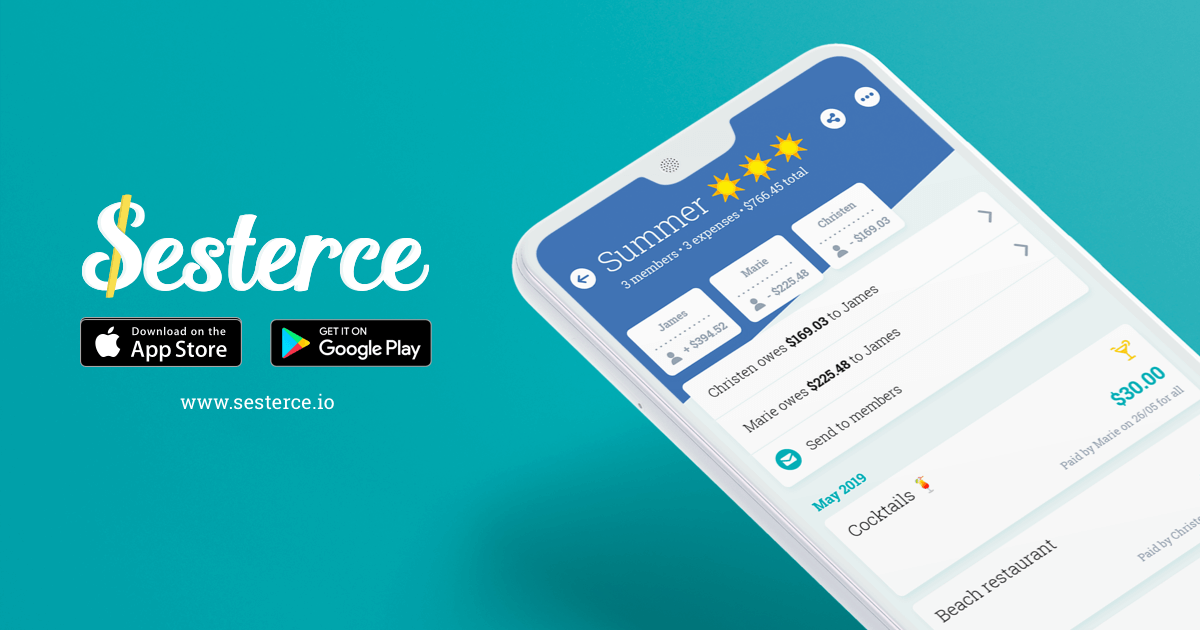
\includegraphics[width=50mm,scale=0.5]{img/logo-sesterce.png}}
            \caption{Sesterce}
            \label{fig:my_label}
        \end{figure}
        \newline
        The setup is pretty similar to create a group and add members.
        \newline
        There's only 1 main screen in Sesterce. It shows the group name, the number of members, the number of expenses, how much money was spent, who owes money or is owed money by whom. It also shows the list of all expenses sorted by date. The expenses display is pretty similar to Tricount as well, showing the title, the amount of the expense, who it is paid by and for whom. You can also add expenses. You have to chose who paid (one or multiple persons), the amount paid by each person, then select a title, add a date and choose a category for the expense (accommodation, groceries, transportation, you can even add your own category).  
\end{enumerate}

\newpage
\section{Specifications}
\begin{enumerate}
    \item \textbf {Loading Screen}
        \begin{figure}[h!]
            \centerline{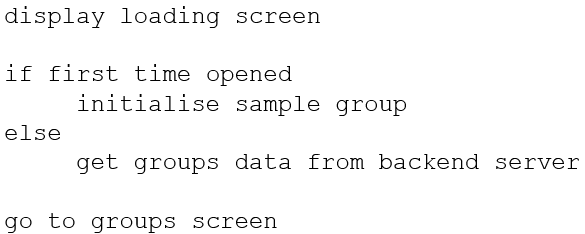
\includegraphics[width=50mm,scale=0.5]{img/pseudocode/pseudocode-loading.png}}
            \caption{Loading Screen Pseudocode}
            \label{fig:my_label}
        \end{figure}
    \item \textbf {Groups}:
        \begin{figure}[h!]
            \centerline{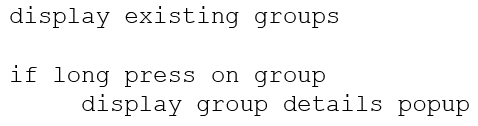
\includegraphics[width=50mm,scale=0.5]{img/pseudocode/pseudocode-groups.png}}
            \caption{Groups Pseudocode}
            \label{fig:my_label}
        \end{figure}
        \begin{enumerate}
            \item \textbf{Enter Group}:
                \begin{figure}[h!]
                    \centerline{
\includegraphics[width=50mm,scale=0.5]{img/pseudocode/pseudocode-enter_group.png}}
                    \caption{Enter Group Pseudocode}
                    \label{fig:my_label}
                \end{figure}
            \item \textbf {Add Group}:
                \begin{figure}[h!]
                    \centerline{
\includegraphics[width=50mm,scale=0.5]{img/pseudocode/pseudocode-add_group.png}}
                    \caption{Add Group Pseudocode}
                    \label{fig:my_label}
                \end{figure}
                \begin{enumerate}
                    \item\textbf {Make New Group}:
                        \begin{figure}[h!]
                            \centerline{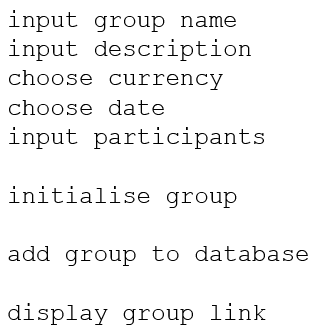
\includegraphics[width=50mm,scale=0.5]{img/pseudocode/pseudocode-make_group.png}}
                            \caption{Make New Group Pseudocode}
                            \label{fig:my_label}
                        \end{figure}
                        \newline \newline \newline \newline \newline \newline \newline \newline
                        \newline \newline
                    \item\textbf {Join Group}:
                        \begin{figure}[h!]
                            \centerline{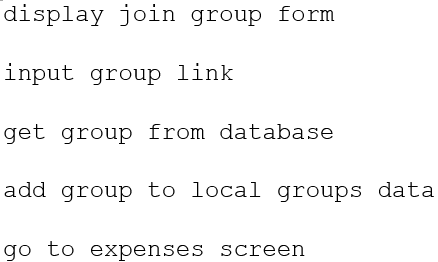
\includegraphics[width=50mm,scale=0.5]{img/pseudocode/pseudocode-join_group.png}}
                            \caption{Join Group Pseudocode}
                            \label{fig:my_label}
                        \end{figure}
                \end{enumerate}
                \item \textbf{Edit Group}
                    \begin{figure}[h!]
                        \centerline{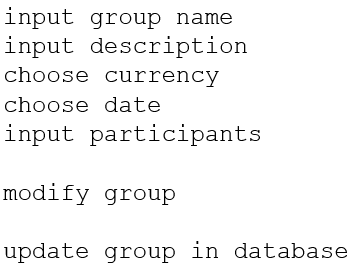
\includegraphics[width=50mm,scale=0.5]{img/pseudocode/pseudocode-edit_group.png}}
                        \caption{Edit Group Pseudocode}
                        \label{fig:my_label}
                    \end{figure}
                \item \textbf{Delete Group}
                    \begin{figure}[h!]
                        \centerline{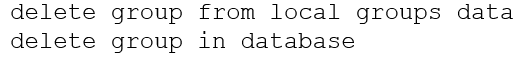
\includegraphics[width=50mm,scale=0.5]{img/pseudocode/pseudocode-delete_group.png}}
                        \caption{Delete Group Pseudocode}
                        \label{fig:my_label}
                    \end{figure}
        \end{enumerate}
    \item \textbf {Expenses}
        \begin{figure}[h!]
            \centerline{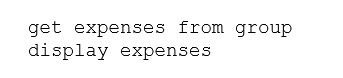
\includegraphics[width=50mm,scale=0.5]{img/pseudocode/pseudocode-expenses.jpg}}
            \caption{Expenses Pseudocode}
            \label{fig:my_label}
        \end{figure}
        \newpage
        \begin{enumerate}
            \item \textbf{Add Expense}
                \begin{figure}[h!]
                    \centerline{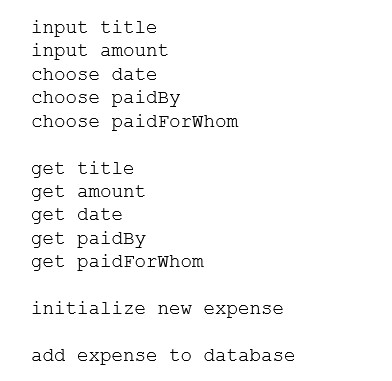
\includegraphics[width=50mm,scale=0.5]{img/pseudocode/pseudocode-add_expense.jpg}}
                    \caption{Add Expense Pseudocode}
                    \label{fig:my_label}
                \end{figure}
            \item \textbf{Expense Detail}
                \begin{figure}[h!]
                    \centerline{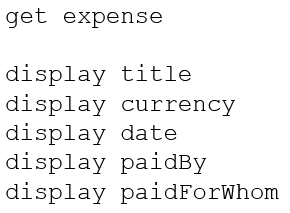
\includegraphics[width=50mm,scale=0.5]{img/pseudocode/pseudocode-expense.png}}
                    \caption{Expense Details Pseudocode}
                    \label{fig:my_label}
                \end{figure}
            \item \textbf{Edit Expense}
                \begin{figure}[h!]
                    \centerline{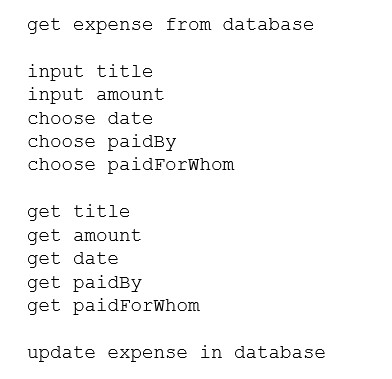
\includegraphics[width=50mm,scale=0.5]{img/pseudocode/pseudocode-edit_expense.jpg}}
                    \caption{Edit Expense Pseudocode}
                    \label{fig:my_label}
                \end{figure}
            \item \textbf{Delete Expense}
                \begin{figure}[h!]
                    \centerline{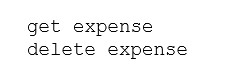
\includegraphics[width=50mm,scale=0.5]{img/pseudocode/pseudocode-delete_expense.jpg}}
                    \caption{Delete Expense Pseudocode}
                    \label{fig:my_label}
                \end{figure}
                \newline \newline
        \end{enumerate}
    \item \textbf{Balances}
        \newline
        \begin{figure}[h!]
            \centerline{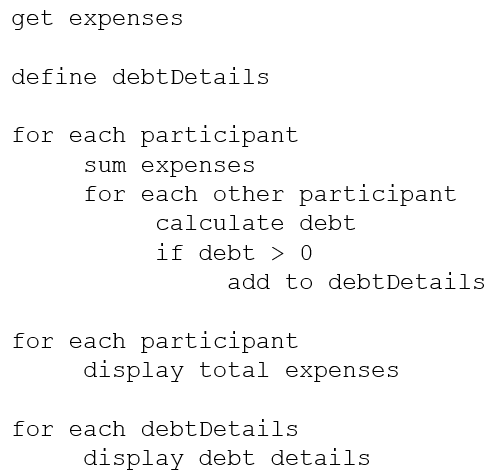
\includegraphics[width=50mm,scale=0.5]{img/pseudocode/pseudocode-balances.png}}
            \caption{Balances Pseudocode}
            \label{fig:my_label}
        \end{figure}
    \end{enumerate}

\end{document}
